\documentclass[12pt]{article}
\usepackage{fullpage,enumitem,amsmath,amssymb,graphicx}
\usepackage{ctex}
\usepackage{multicol}
\usepackage{titlesec}
\usepackage{booktabs}
\usepackage{threeparttable}
\titleformat{\subsubsection}[runin]{\bfseries}{}{}{}[]


\title{贪吃蛇大作业报告}
\author{郑立言 \\
	2016011324\\
	 \texttt{zhengly123@outlook.com}\\
	 \texttt{TEL/WeChat:13362756681}}

\begin{document}
  \maketitle
  \rule{\linewidth}{0.4pt}
  
  \section{设计架构}
  本作业采用了Server-Client模式,需要一个单独的服务器,在服务器开启后,所有的客户端向服务器发起连接。总体来说,使用这一模式的好处有
  \begin{itemize}
  	\item 可以支持多人、多房间对战,扩展性好
  	\item 玩家间同步方便,有唯一的标准
  \end{itemize}
  
  本作业利用帧同步技术,将每一帧地图都发送到各个客户端。这样可以减小客户端的负担,从任何时刻都可以直接同步到当前状态。由于游戏中信息较少,经过测试这种设计能够较好运行。
 
 为了减少各模块依赖,作业采用了将所有MVC模式中的Model、Controller部分放在服务器中,将View部分放在客户端中。
  
  \subsection*{服务器架构}
  
  服务器负责接受客户端的键盘事件、处理游戏逻辑、发送每一时刻的地图到各个客户端。
  结合图 \ref{fig:servercg} ,可以看到程序从StartWindow开始,然后建立ServerMainController进行服务器控制,对于每个连接的用户,建立ServerPeerSocket进行异步通讯。在进入房间时,建立GameController,并将控制权转交给其进行。待玩家全部就绪,游戏开始时,创建ServerGameSocket进行游戏内容通讯。
\begin{figure}[h]
\centering
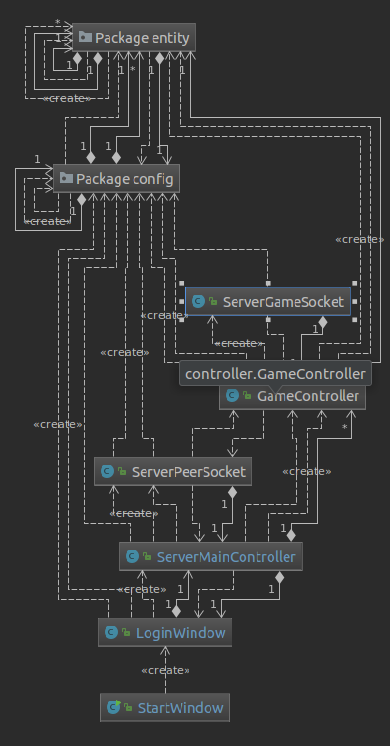
\includegraphics[width=0.7\linewidth]{servercg}
\caption{服务器类图(entity与config中为消息类与地图相关的类)}
\label{fig:servercg}
\end{figure}

\subsection*{客户端架构}

  客户端负责将客户端的键盘事件发送给服务器,接受服务器发送的地图数据并呈现给用户。
  
  结合图 \ref{fig:clientcg} 可以看到,客户端的逻辑较为简单,通过ClientSocket接受数据,并接受窗体触发的事件发送给服务器。

\begin{figure}[h]
\centering
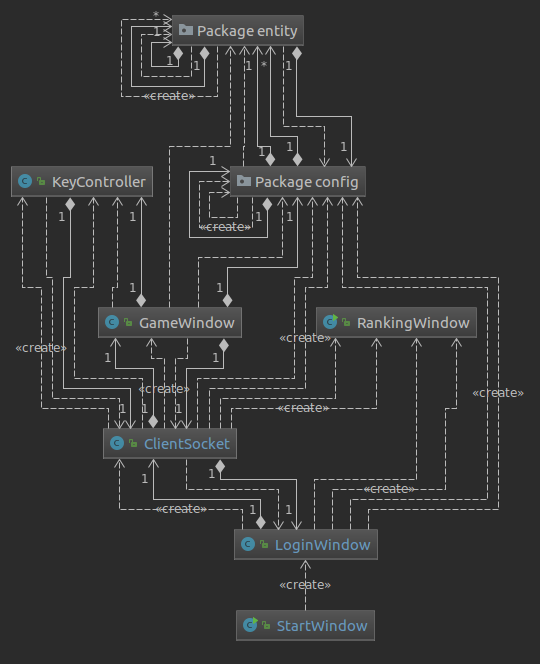
\includegraphics[width=0.7\linewidth]{clientcg}
\caption{客户端类图}
\label{fig:clientcg}
\end{figure}

  \section{模块设计}
   
  \subsection*{UI与数据的交互}
  对服务端而言,ServerMainController和GameController负责逻辑事物。所有Socket接受到的信息都要通知Controller,而后由Controller进行转发等操作,数据也都会经过Controller。这样做使得Socket的设计较为独立,可以方便的处理新的消息类型,解耦合了Socket与具体操作的关联。
  
  对客户端而言,UI与通讯处在两个线程,因此,UI触发的事件需要通过调用ClientSocket进行通讯。而ClientSocket接受到数据时,通过调用UI的成员函数进行展示,两者存在强耦合关系。
  
  \subsection*{碰撞检测}
  贪吃蛇游戏逻辑非常复杂,尤其是碰撞检测环节,有多种可能性,在大于两名玩家的情况下更加突出。
  
  为了方便处理,我采用了先将所有的蛇根据用户输入进行移动,然后再判断有无碰撞。可以发现,在这种情况下,只有蛇头可能与其他蛇发生碰撞,也只用对移动后的地图中,所有物体进行检测有无重叠。
  
  首先需要检测的是蛇有无吃蛋,有的话则将蛇长度加一(这里可能有两只蛇同时吃一个蛋)。然后再判断有无蛇头与其他蛇或墙发生碰撞。最后,将所有的有碰撞的蛇删去,就得到了下一个时刻的地图。
  
  相反的,如果采用对每只蛇进行移动,然后判断,会非常繁琐,需要考虑连锁反应与时间差。
  
  \subsection*{同步机制与网络通讯}
  由于每次通讯只需要发送蛇、蛋等信息,因此信息量较小。每个时刻,服务器将地图中的可变信息发送给客户端,然后客户端进行更新展示。
  因此客户端即使收到了有延迟的消息,在延迟消失后,也会直接进入到最新状态,实现同步。
  在这种情况下,由于客户端没有任何逻辑计算,只有服务器唯一一个状态,能够方便进行同步。理论上即使客户端掉线,重连后还能继续游戏。
  
  网络通讯使用了ObjectOutputStream与ObjectInputStream,发送序列化后的对象,避免了字符串编码带来的粘包等问题。
  
  \section{设计思路}
  
  \subsubsection*{逻辑与通讯分离}
  在最初的设计中,我首先完成了一个单机版的单人贪吃蛇,确保了所有的游戏逻辑正确。这样之后,加上网络通讯部分,可以提前排除游戏逻辑的错误,减小调试的难度。
  
  \subsubsection*{界面与逻辑分离}
  在作业中,受益于用户界面(客户端中的Window)与逻辑(服务器中的Controller)的完全分离,我使用了绝大部分时间开发逻辑部分,仅仅使用一天就完成了所有用户界面。
  
  \subsubsection*{使用一个JPanel进行绘制}
  在Linux平台上,使用较多的JPanel进行绘画操作,会导致界面刷新不一致,例如图 \ref{fig:linux} 。但这一问题在Windows下并不严重。这可能是因为Linux中的可视化库效率较低导致的。
  
  \section{其他}
  感谢助教在小学期中的辛勤付出,您是我遇到的最耐心的助教啦$\sim$ 
\begin{figure}[h]
\centering
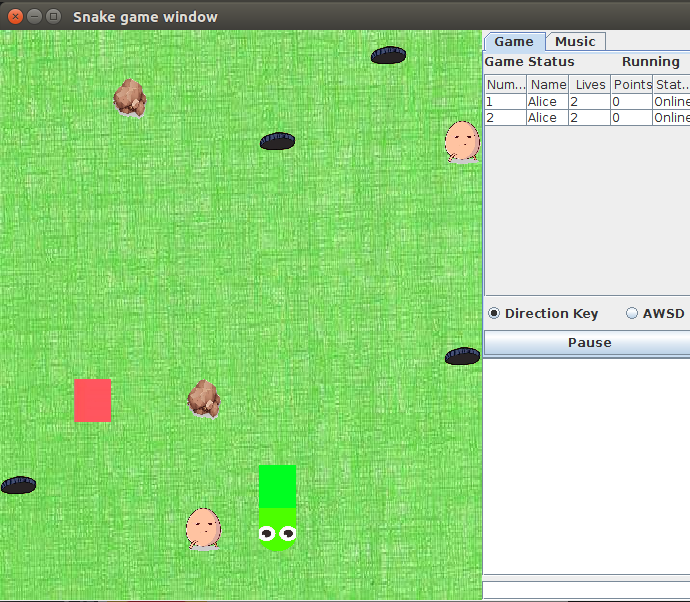
\includegraphics[width=0.7\linewidth]{linux}
\caption{Linux下多个JPanel刷新不同步,左侧蛇头消失}
\label{fig:linux}
\end{figure}
  
\end{document}